\documentclass{beamer}
\usepackage{progressbar, tcolorbox, CJKutf8, hyperref, multicol, pdfpages, graphicx, xcolor, blindtext, tikz, smartdiagram, listings}
\usepackage[absolute,overlay]{textpos}
\usepackage[backend=bibtex,style=numeric,sorting=none]{biblatex}

\hypersetup{
    colorlinks=true,
    linkcolor=blue,
    filecolor=magenta,      
    urlcolor=blue,
    }

    \definecolor{mygreen}{rgb}{0,0.6,0}
    \definecolor{mygray}{rgb}{0.5,0.5,0.5}
    \definecolor{mymauve}{rgb}{0.58,0,0.82}


    \lstset{ 
      backgroundcolor=\color{white},   % choose the background color; you must add \usepackage{color} or \usepackage{xcolor}; should come as last argument
      basicstyle=\ttfamily\footnotesize,% the size of the fonts that are used for the code
      breakatwhitespace=false,         % sets if automatic breaks should only happen at whitespace
      breaklines=true,                 % sets automatic line breaking
      captionpos=b,                    % sets the caption-position to bottom
      commentstyle=\color{mygreen},    % comment style
      deletekeywords={...},            % if you want to delete keywords from the given language
      escapeinside={\%*}{*)},          % if you want to add LaTeX within your code
      extendedchars=true,              % lets you use non-ASCII characters; for 8-bits encodings only, does not work with UTF-8
      frame=single,	                   % adds a frame around the code
      keepspaces=true,                 % keeps spaces in text, useful for keeping indentation of code (possibly needs columns=flexible)
      keywordstyle=\color{magenta},        % keyword style
      morekeywords={FROM, RUN, ENV, USER, WORKDIR, CMD, EXPOSE, ADD, COPY, sudo, curl, chmod, ln, git, cd},
                                       % if you want to add more keywords to the set
      numbers=left,                    % where to put the line-numbers; possible values are (none, left, right)
      numbersep=5pt,                   % how far the line-numbers are from the code
      numberstyle=\tiny\color{mygray}, % the style that is used for the line-numbers
      rulecolor=\color{black},         % if not set, the frame-color may be changed on line-breaks within not-black text (e.g. comments (green here))
      showspaces=false,                % show spaces everywhere adding particular underscores; it overrides 'showstringspaces'
      showstringspaces=false,          % underline spaces within strings only
      showtabs=false,                  % show tabs within strings adding particular underscores
      stepnumber=1,                    % the step between two line-numbers. If it's 1, each line will be numbered
      stringstyle=\color{mymauve},     % string literal style
      tabsize=4,	                     % sets default tabsize to ˋ spaces
      title=\lstname
    }

\graphicspath{ {./images/} }
\usetheme{AnnArbor}
\addbibresource{main.bib}
\usetikzlibrary{positioning, calc, shapes.multipart, shapes.arrows, fit, backgrounds}

\definecolor{dockerColor}{RGB}{13, 183, 237}
\definecolor{secureColor}{RGB}{10, 191, 83}
\definecolor{aquamarine}{rgb}{0.5, 1.0, 0.83}
\definecolor{aquamarine2}{rgb}{0.2, 1.0, 0.53}

\title{The Container Security in Healthcare Data Exchange System}
\subtitle{Bachelor's degree graduation project}
\author{Chih-Hsuan Yang}
\institute{National Sun Yat-sen University\\
Advisor: Chun-I Fan
}
\date{\today}

\AtBeginSection[]{
  \begin{frame}
  \vfill
  \centering
  \begin{beamercolorbox}[sep=8pt,center,shadow=true,rounded=true]{title}
    \usebeamerfont{title}\insertsectionhead\par%
  \end{beamercolorbox}
  \vfill
  \end{frame}
}

\def\checkmark{\tikz\fill[scale=0.4](0,.35) -- (.25,0) -- (1,.7) -- (.25,.15) -- cycle;} 

\begin{document}
\begin{CJK*}{UTF8}{bsmi}

  \begin{frame}
    \titlepage
  \end{frame}


  \begin{frame}{Outline}
    \begin{multicols}{2}
      \tableofcontents
    \end{multicols}
  \end{frame}

  \begin{frame}{Flow chart}
    \centering
    \scalebox{0.9} {
      \smartdiagram[flow diagram:horizontal]{
        Scan base, Sign, Image checking, Start policy, Runtime enforcement
      }
    }
  \end{frame}

  \section{TL;DR}
  \begin{frame}{Current state}
    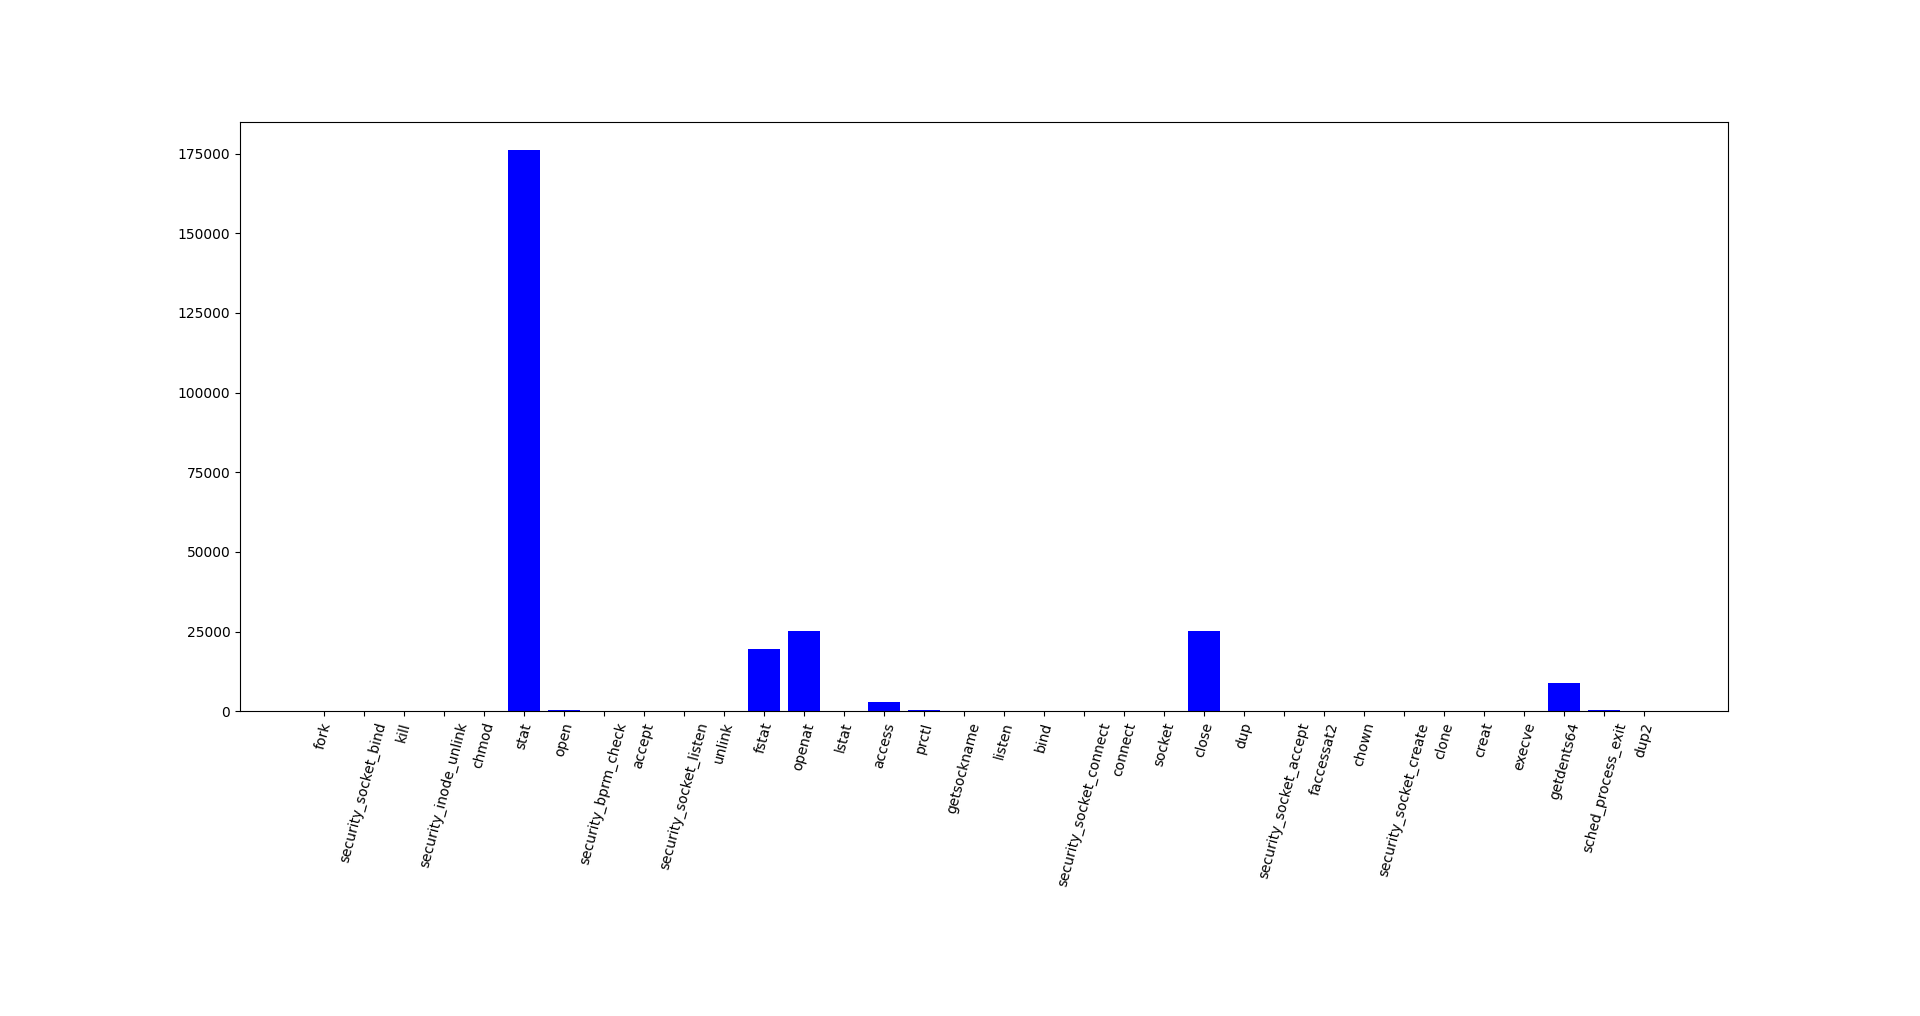
\includegraphics[width=\textwidth]{hist.png}
  \end{frame}

  \begin{frame}{Current state}
    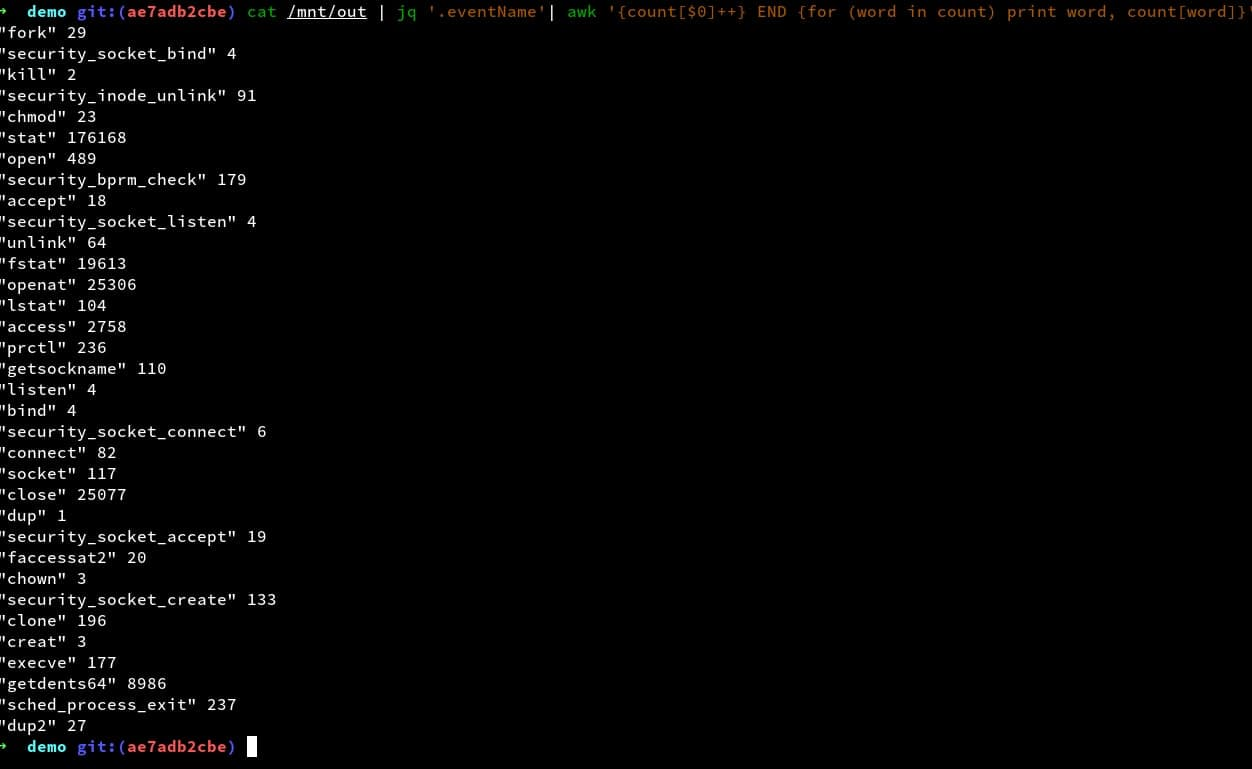
\includegraphics[width=\textwidth]{photo_2021-09-10_14-04-18.jpg}
  \end{frame}

  \begin{frame}{Current state}
    \centering
    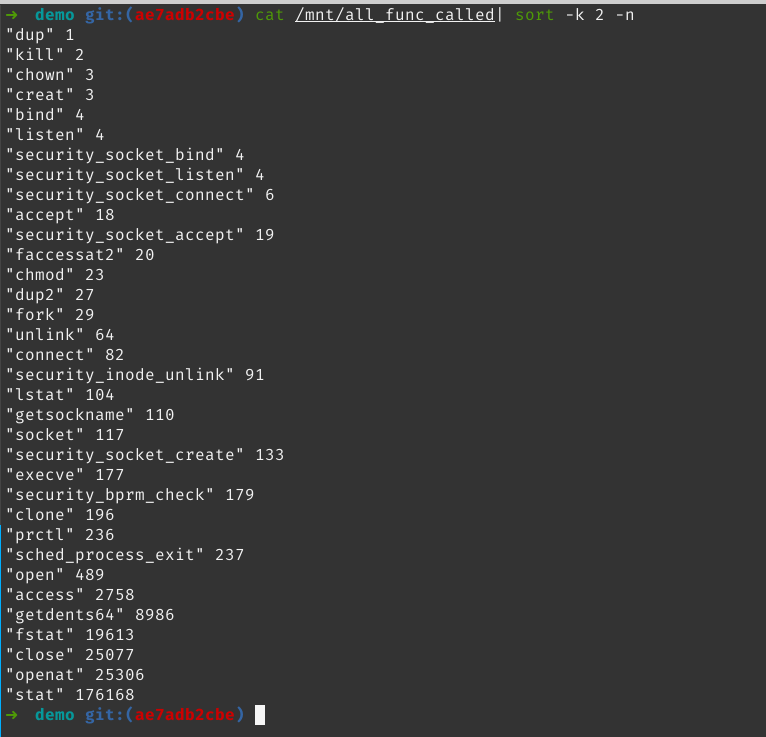
\includegraphics[height=.8\textheight]{Screenshot_2021-09-10_15-15-13.png}
  \end{frame}

  \begin{frame}{Problems}
    \begin{enumerate}
      \item How to demonstrate in {\color{blue} demo day}, in {\color{blue} paper}?
            \begin{enumerate}
              \item Might not have those attacking dataset. (Ask stavhaygn)
              \item For some specialized attacks? (BOF, DOS)?
              \item Infrastructure threats.
            \end{enumerate}
      \item We do not reject the performance is same as the raw system.
      \item Some other protection surface?
    \end{enumerate}
  \end{frame}

  \section{Screenshots}

  \begin{frame}{Unitests and intergration tests}
    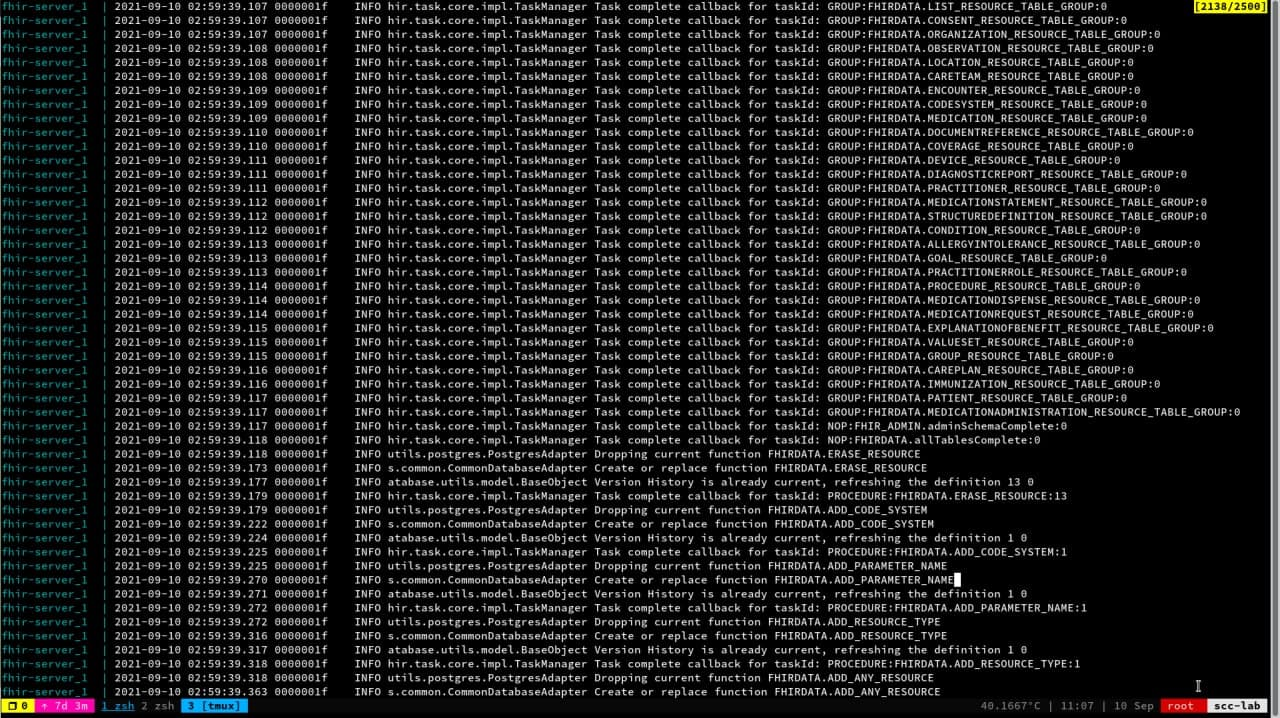
\includegraphics[width=\textwidth]{photo_2021-09-10_14-04-02.jpg}
  \end{frame}

  \begin{frame}
    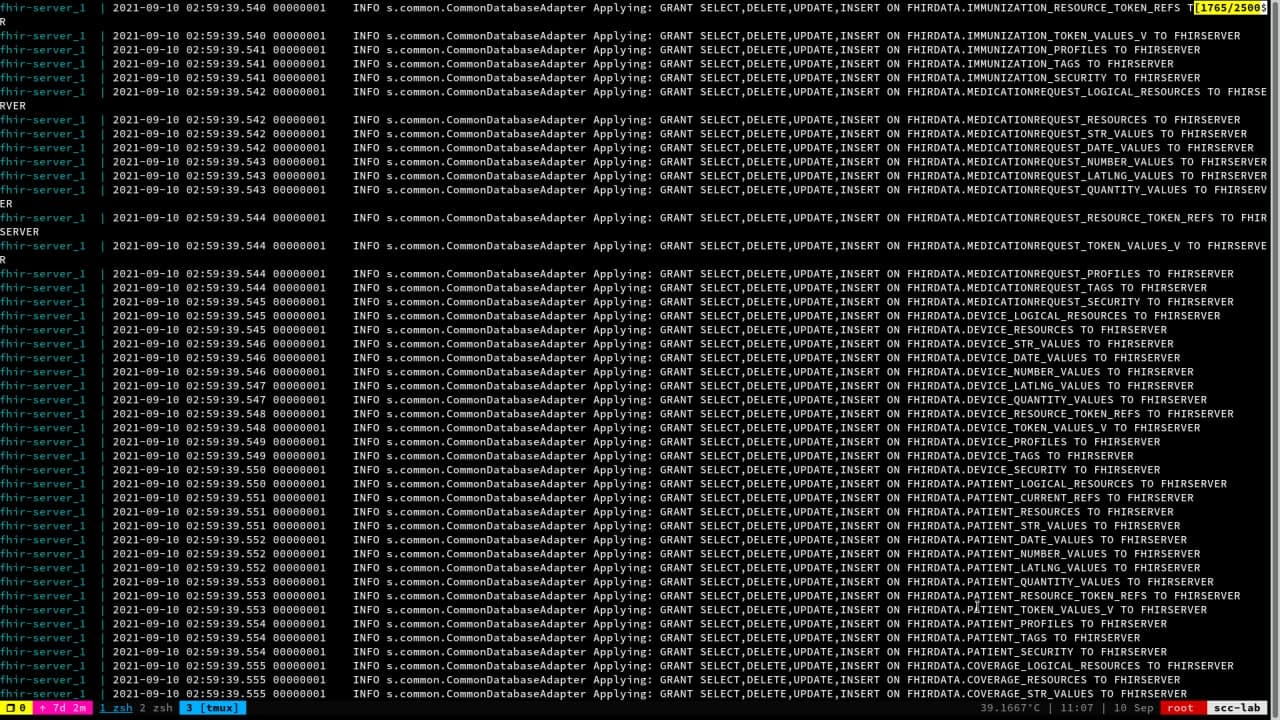
\includegraphics[width=\textwidth]{photo_2021-09-10_14-03-57.jpg}
  \end{frame}

  \begin{frame}
    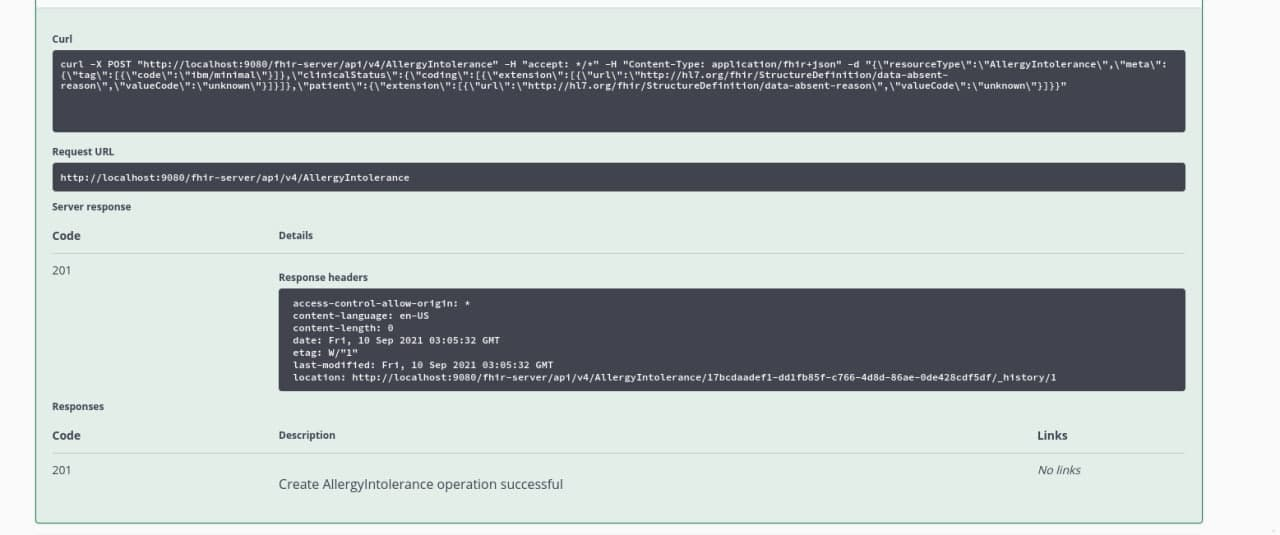
\includegraphics[width=\textwidth]{photo_2021-09-10_14-03-44.jpg}
    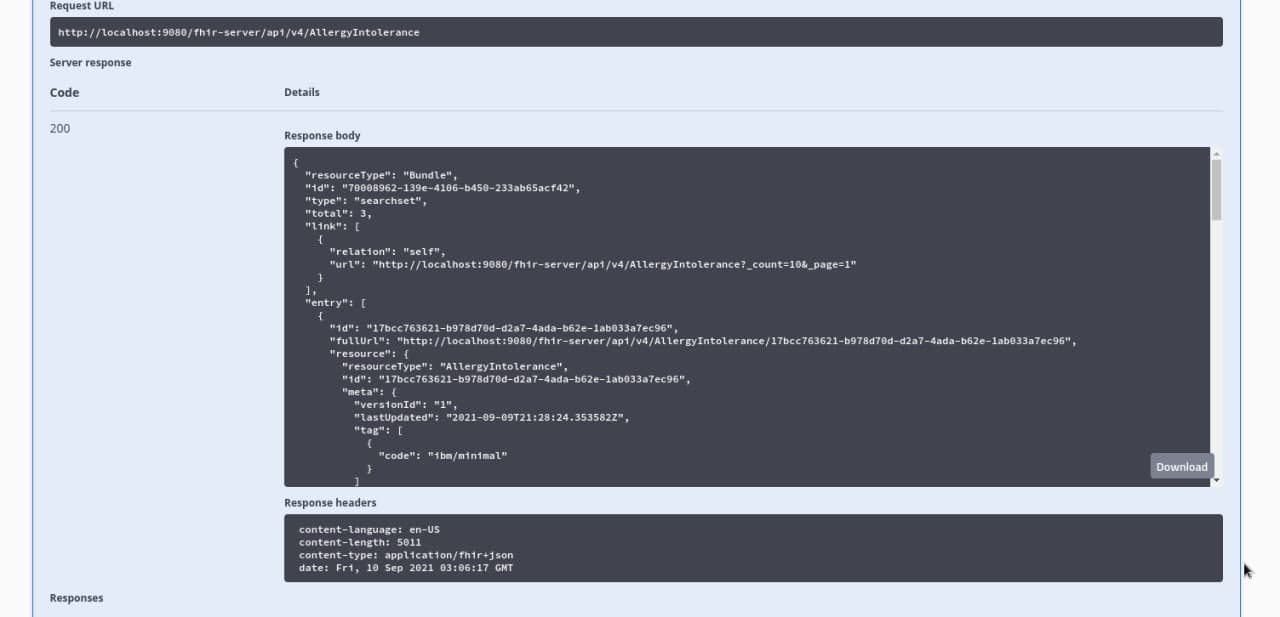
\includegraphics[width=\textwidth]{photo_2021-09-10_14-03-52.jpg}
  \end{frame}

  \begin{frame}
    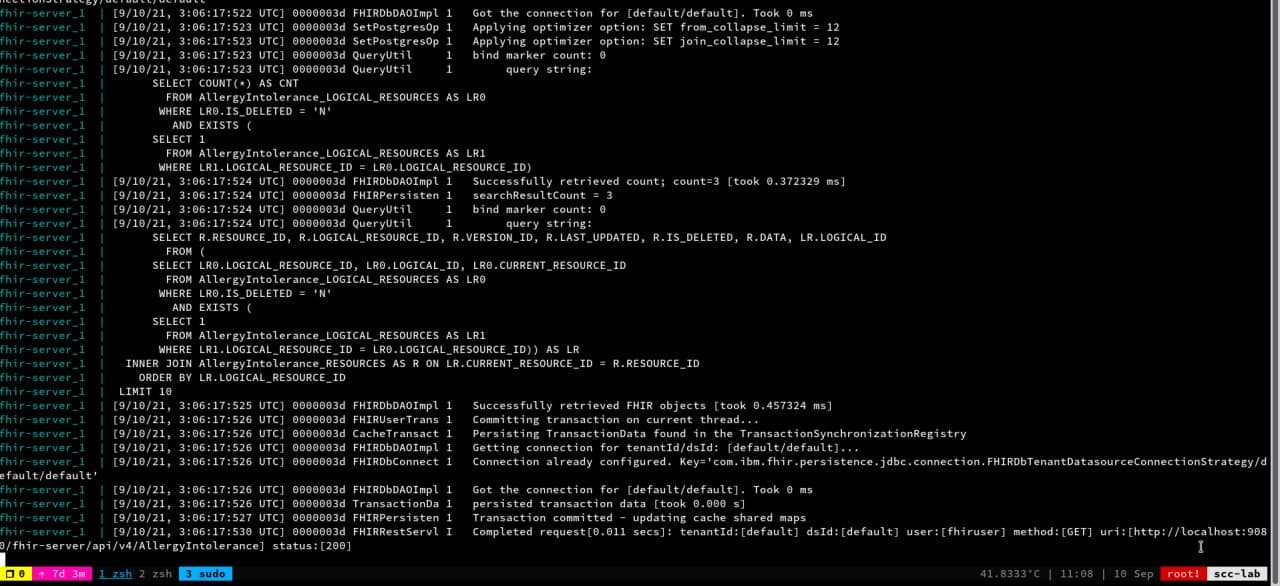
\includegraphics[width=\textwidth]{photo_2021-09-10_14-04-10.jpg}
  \end{frame}

  \begin{frame}
    \begin{multicols*}{2}
      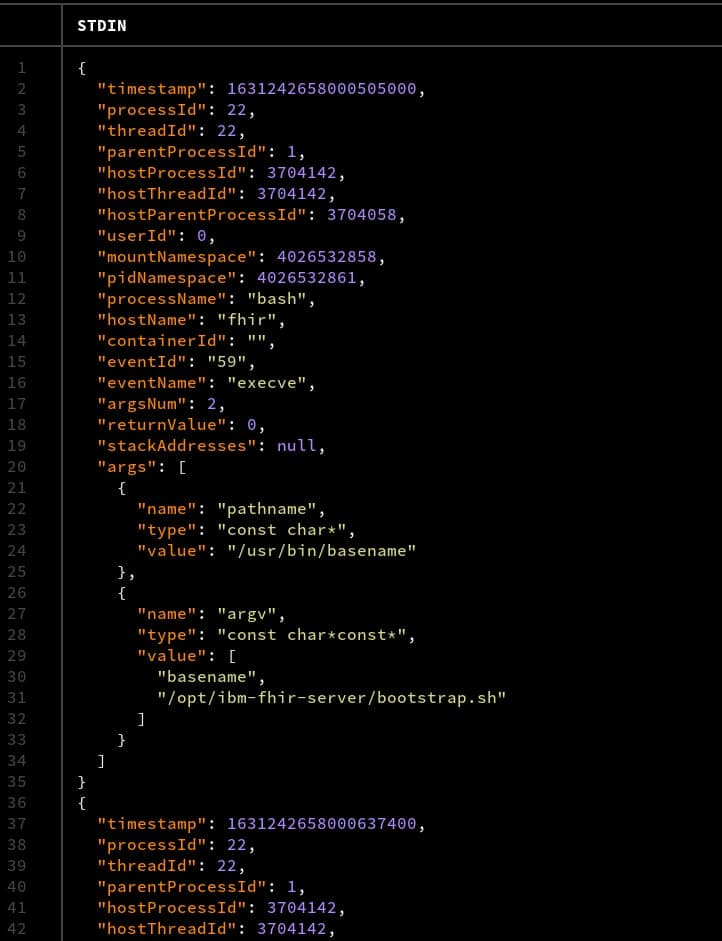
\includegraphics[height=.9\textheight]{photo_2021-09-10_14-04-25.jpg}
      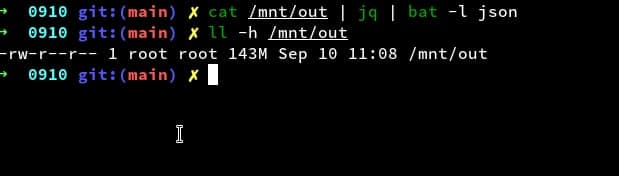
\includegraphics[width=.45\textwidth]{photo_2021-09-10_14-04-30.jpg}
    \end{multicols*}
  \end{frame}

  \begin{frame}{Problems}
    \begin{enumerate}
      \item How to demonstrate in {demo day}, in {paper}?
            \begin{enumerate}
              \item Might not have those attacking dataset. (Ask stavhaygn)
              \item For some specialized attacks? (BOF, DOS)?
              \item Infrastructure threats.
            \end{enumerate}
      \item We do not reject the performance is same as the raw system.
      \item Some {\color{red} other protection surface}?
    \end{enumerate}
  \end{frame}

\end{CJK*}
\end{document}